\documentclass[1p]{elsarticle_modified}
%\bibliographystyle{elsarticle-num}

%\usepackage[colorlinks]{hyperref}
%\usepackage{abbrmath_seonhwa} %\Abb, \Ascr, \Acal ,\Abf, \Afrak
\usepackage{amsfonts}
\usepackage{amssymb}
\usepackage{amsmath}
\usepackage{amsthm}
\usepackage{scalefnt}
\usepackage{amsbsy}
\usepackage{kotex}
\usepackage{caption}
\usepackage{subfig}
\usepackage{color}
\usepackage{graphicx}
\usepackage{xcolor} %% white, black, red, green, blue, cyan, magenta, yellow
\usepackage{float}
\usepackage{setspace}
\usepackage{hyperref}

\usepackage{tikz}
\usetikzlibrary{arrows}

\usepackage{multirow}
\usepackage{array} % fixed length table
\usepackage{hhline}

%%%%%%%%%%%%%%%%%%%%%
\makeatletter
\renewcommand*\env@matrix[1][\arraystretch]{%
	\edef\arraystretch{#1}%
	\hskip -\arraycolsep
	\let\@ifnextchar\new@ifnextchar
	\array{*\c@MaxMatrixCols c}}
\makeatother %https://tex.stackexchange.com/questions/14071/how-can-i-increase-the-line-spacing-in-a-matrix
%%%%%%%%%%%%%%%

\usepackage[normalem]{ulem}

\newcommand{\msout}[1]{\ifmmode\text{\sout{\ensuremath{#1}}}\else\sout{#1}\fi}
%SOURCE: \msout is \stkout macro in https://tex.stackexchange.com/questions/20609/strikeout-in-math-mode

\newcommand{\cancel}[1]{
	\ifmmode
	{\color{red}\msout{#1}}
	\else
	{\color{red}\sout{#1}}
	\fi
}

\newcommand{\add}[1]{
	{\color{blue}\uwave{#1}}
}

\newcommand{\replace}[2]{
	\ifmmode
	{\color{red}\msout{#1}}{\color{blue}\uwave{#2}}
	\else
	{\color{red}\sout{#1}}{\color{blue}\uwave{#2}}
	\fi
}

\newcommand{\Sol}{\mathcal{S}} %segment
\newcommand{\D}{D} %diagram
\newcommand{\A}{\mathcal{A}} %arc


%%%%%%%%%%%%%%%%%%%%%%%%%%%%%5 test

\def\sl{\operatorname{\textup{SL}}(2,\Cbb)}
\def\psl{\operatorname{\textup{PSL}}(2,\Cbb)}
\def\quan{\mkern 1mu \triangleright \mkern 1mu}

\theoremstyle{definition}
\newtheorem{thm}{Theorem}[section]
\newtheorem{prop}[thm]{Proposition}
\newtheorem{lem}[thm]{Lemma}
\newtheorem{ques}[thm]{Question}
\newtheorem{cor}[thm]{Corollary}
\newtheorem{defn}[thm]{Definition}
\newtheorem{exam}[thm]{Example}
\newtheorem{rmk}[thm]{Remark}
\newtheorem{alg}[thm]{Algorithm}

\newcommand{\I}{\sqrt{-1}}
\begin{document}

%\begin{frontmatter}
%
%\title{Boundary parabolic representations of knots up to 8 crossings}
%
%%% Group authors per affiliation:
%\author{Yunhi Cho} 
%\address{Department of Mathematics, University of Seoul, Seoul, Korea}
%\ead{yhcho@uos.ac.kr}
%
%
%\author{Seonhwa Kim} %\fnref{s_kim}}
%\address{Center for Geometry and Physics, Institute for Basic Science, Pohang, 37673, Korea}
%\ead{ryeona17@ibs.re.kr}
%
%\author{Hyuk Kim}
%\address{Department of Mathematical Sciences, Seoul National University, Seoul 08826, Korea}
%\ead{hyukkim@snu.ac.kr}
%
%\author{Seokbeom Yoon}
%\address{Department of Mathematical Sciences, Seoul National University, Seoul, 08826,  Korea}
%\ead{sbyoon15@snu.ac.kr}
%
%\begin{abstract}
%We find all boundary parabolic representation of knots up to 8 crossings.
%
%\end{abstract}
%\begin{keyword}
%    \MSC[2010] 57M25 
%\end{keyword}
%
%\end{frontmatter}

%\linenumbers
%\tableofcontents
%
\newcommand\colored[1]{\textcolor{white}{\rule[-0.35ex]{0.8em}{1.4ex}}\kern-0.8em\color{red} #1}%
%\newcommand\colored[1]{\textcolor{white}{ #1}\kern-2.17ex	\textcolor{white}{ #1}\kern-1.81ex	\textcolor{white}{ #1}\kern-2.15ex\color{red}#1	}

{\Large $\underline{12a_{0132}~(K12a_{0132})}$}

\setlength{\tabcolsep}{10pt}
\renewcommand{\arraystretch}{1.6}
\vspace{1cm}\begin{tabular}{m{100pt}>{\centering\arraybackslash}m{274pt}}
\multirow{5}{120pt}{
	\centering
	\includegraphics[width=112pt]{../../../GIT/diagram.site/Diagrams/png/933_12a_0132.png}\\
\ \ \ A knot diagram\footnotemark}&
\allowdisplaybreaks
\textbf{Linearized knot diagam} \\
\cline{2-2}
 &
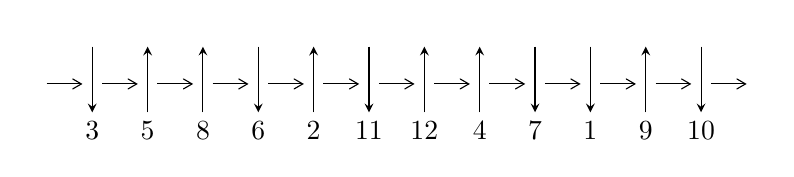
\begin{tikzpicture}[x=20pt, y=17pt]
	% nodes
	\node (C0) at (0, 0) {};
	\node (C1) at (1, 0) {};
	\node (C1U) at (1, +1) {};
	\node (C1D) at (1, -1) {3};

	\node (C2) at (2, 0) {};
	\node (C2U) at (2, +1) {};
	\node (C2D) at (2, -1) {5};

	\node (C3) at (3, 0) {};
	\node (C3U) at (3, +1) {};
	\node (C3D) at (3, -1) {8};

	\node (C4) at (4, 0) {};
	\node (C4U) at (4, +1) {};
	\node (C4D) at (4, -1) {6};

	\node (C5) at (5, 0) {};
	\node (C5U) at (5, +1) {};
	\node (C5D) at (5, -1) {2};

	\node (C6) at (6, 0) {};
	\node (C6U) at (6, +1) {};
	\node (C6D) at (6, -1) {11};

	\node (C7) at (7, 0) {};
	\node (C7U) at (7, +1) {};
	\node (C7D) at (7, -1) {12};

	\node (C8) at (8, 0) {};
	\node (C8U) at (8, +1) {};
	\node (C8D) at (8, -1) {4};

	\node (C9) at (9, 0) {};
	\node (C9U) at (9, +1) {};
	\node (C9D) at (9, -1) {7};

	\node (C10) at (10, 0) {};
	\node (C10U) at (10, +1) {};
	\node (C10D) at (10, -1) {1};

	\node (C11) at (11, 0) {};
	\node (C11U) at (11, +1) {};
	\node (C11D) at (11, -1) {9};

	\node (C12) at (12, 0) {};
	\node (C12U) at (12, +1) {};
	\node (C12D) at (12, -1) {10};
	\node (C13) at (13, 0) {};

	% arrows
	\draw[->,>={angle 60}]
	(C0) edge (C1) (C1) edge (C2) (C2) edge (C3) (C3) edge (C4) (C4) edge (C5) (C5) edge (C6) (C6) edge (C7) (C7) edge (C8) (C8) edge (C9) (C9) edge (C10) (C10) edge (C11) (C11) edge (C12) (C12) edge (C13) ;	\draw[->,>=stealth]
	(C1U) edge (C1D) (C2D) edge (C2U) (C3D) edge (C3U) (C4U) edge (C4D) (C5D) edge (C5U) (C6U) edge (C6D) (C7D) edge (C7U) (C8D) edge (C8U) (C9U) edge (C9D) (C10U) edge (C10D) (C11D) edge (C11U) (C12U) edge (C12D) ;
	\end{tikzpicture} \\
\hhline{~~} \\& 
\textbf{Solving Sequence} \\ \cline{2-2} 
 &
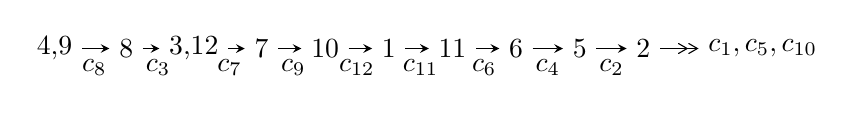
\begin{tikzpicture}[x=23pt, y=7pt]
	% node
	\node (A0) at (-1/8, 0) {4,9};
	\node (A1) at (1, 0) {8};
	\node (A2) at (33/16, 0) {3,12};
	\node (A3) at (25/8, 0) {7};
	\node (A4) at (33/8, 0) {10};
	\node (A5) at (41/8, 0) {1};
	\node (A6) at (49/8, 0) {11};
	\node (A7) at (57/8, 0) {6};
	\node (A8) at (65/8, 0) {5};
	\node (A9) at (73/8, 0) {2};
	\node (C1) at (1/2, -1) {$c_{8}$};
	\node (C2) at (3/2, -1) {$c_{3}$};
	\node (C3) at (21/8, -1) {$c_{7}$};
	\node (C4) at (29/8, -1) {$c_{9}$};
	\node (C5) at (37/8, -1) {$c_{12}$};
	\node (C6) at (45/8, -1) {$c_{11}$};
	\node (C7) at (53/8, -1) {$c_{6}$};
	\node (C8) at (61/8, -1) {$c_{4}$};
	\node (C9) at (69/8, -1) {$c_{2}$};
	\node (A10) at (11, 0) {$c_{1},c_{5},c_{10}$};

	% edge
	\draw[->,>=stealth]	
	(A0) edge (A1) (A1) edge (A2) (A2) edge (A3) (A3) edge (A4) (A4) edge (A5) (A5) edge (A6) (A6) edge (A7) (A7) edge (A8) (A8) edge (A9) ;
	\draw[->>,>={angle 60}]	
	(A9) edge (A10);
\end{tikzpicture} \\ 

\end{tabular} \\

\footnotetext{
The image of knot diagram is generated by the software ``\textbf{Draw programme}" developed by Andrew Bartholomew(\url{http://www.layer8.co.uk/maths/draw/index.htm\#Running-draw}), where we modified some parts for our purpose(\url{https://github.com/CATsTAILs/LinksPainter}).
}\phantom \\ \newline 
\centering \textbf{Ideals for irreducible components\footnotemark of $X_{\text{par}}$} 
 
\begin{align*}
I^u_{1}&=\langle 
5.62500\times10^{507} u^{123}+6.31929\times10^{507} u^{122}+\cdots+2.55470\times10^{510} b-2.21789\times10^{511},\\
\phantom{I^u_{1}}&\phantom{= \langle  }-6.08901\times10^{508} u^{123}-1.58391\times10^{509} u^{122}+\cdots+1.02188\times10^{511} a-1.29482\times10^{512},\\
\phantom{I^u_{1}}&\phantom{= \langle  }u^{124}+u^{123}+\cdots-5120 u+1024\rangle \\
\\
I^v_{1}&=\langle 
a,\;1728 v^9+4936 v^8+9872 v^7-12908 v^6-24680 v^5+34552 v^4+91527 v^3-4936 v^2+3335 b+613,\\
\phantom{I^v_{1}}&\phantom{= \langle  }v^{10}+3 v^9+6 v^8-7 v^7-16 v^6+19 v^5+58 v^4+2 v^3-7 v^2+v+1\rangle \\
\end{align*}
\raggedright * 2 irreducible components of $\dim_{\mathbb{C}}=0$, with total 134 representations.\\
\footnotetext{All coefficients of polynomials are rational numbers. But the coefficients are sometimes approximated in decimal forms when there is not enough margin.}
\newpage
\renewcommand{\arraystretch}{1}
\centering \section*{I. $I^u_{1}= \langle 5.63\times10^{507} u^{123}+6.32\times10^{507} u^{122}+\cdots+2.55\times10^{510} b-2.22\times10^{511},\;-6.09\times10^{508} u^{123}-1.58\times10^{509} u^{122}+\cdots+1.02\times10^{511} a-1.29\times10^{512},\;u^{124}+u^{123}+\cdots-5120 u+1024 \rangle$}
\flushleft \textbf{(i) Arc colorings}\\
\begin{tabular}{m{7pt} m{180pt} m{7pt} m{180pt} }
\flushright $a_{4}=$&$\begin{pmatrix}0\\u\end{pmatrix}$ \\
\flushright $a_{9}=$&$\begin{pmatrix}1\\0\end{pmatrix}$ \\
\flushright $a_{8}=$&$\begin{pmatrix}1\\u^2\end{pmatrix}$ \\
\flushright $a_{3}=$&$\begin{pmatrix}- u\\- u^3+u\end{pmatrix}$ \\
\flushright $a_{12}=$&$\begin{pmatrix}0.00595864 u^{123}+0.0155000 u^{122}+\cdots+16.8620 u+12.6709\\-0.00220183 u^{123}-0.00247360 u^{122}+\cdots-26.2981 u+8.68161\end{pmatrix}$ \\
\flushright $a_{7}=$&$\begin{pmatrix}-0.0324749 u^{123}-0.0607838 u^{122}+\cdots-230.963 u+46.6844\\0.00378830 u^{123}+0.00499386 u^{122}+\cdots+8.89055 u-5.72918\end{pmatrix}$ \\
\flushright $a_{10}=$&$\begin{pmatrix}0.0182618 u^{123}+0.0309327 u^{122}+\cdots+105.201 u-21.3586\\-0.00140036 u^{123}-0.00248372 u^{122}+\cdots+12.7388 u-3.20499\end{pmatrix}$ \\
\flushright $a_{1}=$&$\begin{pmatrix}-0.00690886 u^{123}-0.00829307 u^{122}+\cdots-79.1920 u+29.3712\\-0.00140036 u^{123}-0.00248372 u^{122}+\cdots+12.7388 u-3.20499\end{pmatrix}$ \\
\flushright $a_{11}=$&$\begin{pmatrix}0.00816047 u^{123}+0.0179736 u^{122}+\cdots+43.1601 u+3.98933\\-0.00220183 u^{123}-0.00247360 u^{122}+\cdots-26.2981 u+8.68161\end{pmatrix}$ \\
\flushright $a_{6}=$&$\begin{pmatrix}-0.0106337 u^{123}-0.0146047 u^{122}+\cdots-66.4407 u+24.7488\\0.00372489 u^{123}+0.00631165 u^{122}+\cdots-12.7513 u+4.62242\end{pmatrix}$ \\
\flushright $a_{5}=$&$\begin{pmatrix}0.00761734 u^{123}+0.00955153 u^{122}+\cdots+44.0856 u-14.0585\\0.0119599 u^{123}+0.0204629 u^{122}+\cdots+101.335 u-28.7078\end{pmatrix}$ \\
\flushright $a_{2}=$&$\begin{pmatrix}-0.00597755 u^{123}-0.00670190 u^{122}+\cdots-69.7496 u+25.3049\\-0.00252974 u^{123}-0.00392118 u^{122}+\cdots+5.72123 u+0.185587\end{pmatrix}$\\&\end{tabular}
\flushleft \textbf{(ii) Obstruction class $= -1$}\\~\\
\flushleft \textbf{(iii) Cusp Shapes $= -0.0208807 u^{123}-0.0235904 u^{122}+\cdots-165.877 u+74.8282$}\\~\\
\newpage\renewcommand{\arraystretch}{1}
\flushleft \textbf{(iv) u-Polynomials at the component}\newline \\
\begin{tabular}{m{50pt}|m{274pt}}
Crossings & \hspace{64pt}u-Polynomials at each crossing \\
\hline $$\begin{aligned}c_{1},c_{4}\end{aligned}$$&$\begin{aligned}
&u^{124}+42 u^{123}+\cdots+2 u+1
\end{aligned}$\\
\hline $$\begin{aligned}c_{2},c_{5}\end{aligned}$$&$\begin{aligned}
&u^{124}+6 u^{123}+\cdots+2 u+1
\end{aligned}$\\
\hline $$\begin{aligned}c_{3},c_{8}\end{aligned}$$&$\begin{aligned}
&u^{124}- u^{123}+\cdots+5120 u+1024
\end{aligned}$\\
\hline $$\begin{aligned}c_{6}\end{aligned}$$&$\begin{aligned}
&u^{124}+3 u^{123}+\cdots-376993 u-48793
\end{aligned}$\\
\hline $$\begin{aligned}c_{7}\end{aligned}$$&$\begin{aligned}
&u^{124}-3 u^{123}+\cdots+1975 u+1031
\end{aligned}$\\
\hline $$\begin{aligned}c_{9}\end{aligned}$$&$\begin{aligned}
&u^{124}-9 u^{123}+\cdots-3 u+1
\end{aligned}$\\
\hline $$\begin{aligned}c_{10},c_{12}\end{aligned}$$&$\begin{aligned}
&u^{124}-3 u^{123}+\cdots-17 u+1
\end{aligned}$\\
\hline $$\begin{aligned}c_{11}\end{aligned}$$&$\begin{aligned}
&u^{124}+21 u^{123}+\cdots+3 u+1
\end{aligned}$\\
\hline
\end{tabular}\\~\\
\newpage\renewcommand{\arraystretch}{1}
\flushleft \textbf{(v) Riley Polynomials at the component}\newline \\
\begin{tabular}{m{50pt}|m{274pt}}
Crossings & \hspace{64pt}Riley Polynomials at each crossing \\
\hline $$\begin{aligned}c_{1},c_{4}\end{aligned}$$&$\begin{aligned}
&y^{124}+86 y^{123}+\cdots-1250 y+1
\end{aligned}$\\
\hline $$\begin{aligned}c_{2},c_{5}\end{aligned}$$&$\begin{aligned}
&y^{124}+42 y^{123}+\cdots+2 y+1
\end{aligned}$\\
\hline $$\begin{aligned}c_{3},c_{8}\end{aligned}$$&$\begin{aligned}
&y^{124}-55 y^{123}+\cdots-26214400 y+1048576
\end{aligned}$\\
\hline $$\begin{aligned}c_{6}\end{aligned}$$&$\begin{aligned}
&y^{124}+83 y^{123}+\cdots-318551403169 y+2380756849
\end{aligned}$\\
\hline $$\begin{aligned}c_{7}\end{aligned}$$&$\begin{aligned}
&y^{124}+131 y^{123}+\cdots+138554707 y+1062961
\end{aligned}$\\
\hline $$\begin{aligned}c_{9}\end{aligned}$$&$\begin{aligned}
&y^{124}-21 y^{123}+\cdots-9 y+1
\end{aligned}$\\
\hline $$\begin{aligned}c_{10},c_{12}\end{aligned}$$&$\begin{aligned}
&y^{124}-85 y^{123}+\cdots-17 y+1
\end{aligned}$\\
\hline $$\begin{aligned}c_{11}\end{aligned}$$&$\begin{aligned}
&y^{124}+3 y^{123}+\cdots-17 y+1
\end{aligned}$\\
\hline
\end{tabular}\\~\\
\newpage\flushleft \textbf{(vi) Complex Volumes and Cusp Shapes}
$$\begin{array}{c|c|c}  
\text{Solutions to }I^u_{1}& \I (\text{vol} + \sqrt{-1}CS) & \text{Cusp shape}\\
 \hline 
\begin{aligned}
u &= -0.522189 + 0.849715 I \\
a &= \phantom{-}0.0863169 + 0.0937477 I \\
b &= \phantom{-}0.822352 + 1.127080 I\end{aligned}
 & -7.69575 + 7.07073 I & \phantom{-0.000000 } 0 \\ \hline\begin{aligned}
u &= -0.522189 - 0.849715 I \\
a &= \phantom{-}0.0863169 - 0.0937477 I \\
b &= \phantom{-}0.822352 - 1.127080 I\end{aligned}
 & -7.69575 - 7.07073 I & \phantom{-0.000000 } 0 \\ \hline\begin{aligned}
u &= -0.761135 + 0.655567 I \\
a &= \phantom{-}1.73888 + 1.08981 I \\
b &= \phantom{-}1.38408 - 0.94824 I\end{aligned}
 & -6.14991 - 0.54757 I & \phantom{-0.000000 } 0 \\ \hline\begin{aligned}
u &= -0.761135 - 0.655567 I \\
a &= \phantom{-}1.73888 - 1.08981 I \\
b &= \phantom{-}1.38408 + 0.94824 I\end{aligned}
 & -6.14991 + 0.54757 I & \phantom{-0.000000 } 0 \\ \hline\begin{aligned}
u &= \phantom{-}0.890683 + 0.466793 I \\
a &= \phantom{-}1.38896 - 0.33416 I \\
b &= \phantom{-}0.294252 + 0.387769 I\end{aligned}
 & -1.73197 + 2.72965 I & \phantom{-0.000000 } 0 \\ \hline\begin{aligned}
u &= \phantom{-}0.890683 - 0.466793 I \\
a &= \phantom{-}1.38896 + 0.33416 I \\
b &= \phantom{-}0.294252 - 0.387769 I\end{aligned}
 & -1.73197 - 2.72965 I & \phantom{-0.000000 } 0 \\ \hline\begin{aligned}
u &= \phantom{-}0.797869 + 0.557988 I \\
a &= -3.22687 - 0.82452 I \\
b &= -0.405742 + 0.130680 I\end{aligned}
 & -3.73679 + 2.23882 I & \phantom{-0.000000 } 0 \\ \hline\begin{aligned}
u &= \phantom{-}0.797869 - 0.557988 I \\
a &= -3.22687 + 0.82452 I \\
b &= -0.405742 - 0.130680 I\end{aligned}
 & -3.73679 - 2.23882 I & \phantom{-0.000000 } 0 \\ \hline\begin{aligned}
u &= -1.03358\phantom{ +0.000000I} \\
a &= \phantom{-}1.17878\phantom{ +0.000000I} \\
b &= \phantom{-}0.419420\phantom{ +0.000000I}\end{aligned}
 & \phantom{-}1.67471\phantom{ +0.000000I} & \phantom{-0.000000 } 0 \\ \hline\begin{aligned}
u &= \phantom{-}0.152273 + 0.950799 I \\
a &= \phantom{-}0.439586 + 0.095214 I \\
b &= \phantom{-}0.352639 - 0.121692 I\end{aligned}
 & \phantom{-}0.94696 - 2.64839 I & \phantom{-0.000000 } 0\\
 \hline 
 \end{array}$$\newpage$$\begin{array}{c|c|c}  
\text{Solutions to }I^u_{1}& \I (\text{vol} + \sqrt{-1}CS) & \text{Cusp shape}\\
 \hline 
\begin{aligned}
u &= \phantom{-}0.152273 - 0.950799 I \\
a &= \phantom{-}0.439586 - 0.095214 I \\
b &= \phantom{-}0.352639 + 0.121692 I\end{aligned}
 & \phantom{-}0.94696 + 2.64839 I & \phantom{-0.000000 } 0 \\ \hline\begin{aligned}
u &= \phantom{-}0.111280 + 0.950958 I \\
a &= \phantom{-}0.0891030 - 0.0899186 I \\
b &= \phantom{-}0.632776 - 0.873813 I\end{aligned}
 & -4.19980 - 4.72472 I & \phantom{-0.000000 } 0 \\ \hline\begin{aligned}
u &= \phantom{-}0.111280 - 0.950958 I \\
a &= \phantom{-}0.0891030 + 0.0899186 I \\
b &= \phantom{-}0.632776 + 0.873813 I\end{aligned}
 & -4.19980 + 4.72472 I & \phantom{-0.000000 } 0 \\ \hline\begin{aligned}
u &= \phantom{-}0.402887 + 0.866992 I \\
a &= \phantom{-}0.0821980 + 0.0901132 I \\
b &= \phantom{-}0.214260 + 0.899169 I\end{aligned}
 & -7.15417 + 1.85942 I & \phantom{-0.000000 } 0 \\ \hline\begin{aligned}
u &= \phantom{-}0.402887 - 0.866992 I \\
a &= \phantom{-}0.0821980 - 0.0901132 I \\
b &= \phantom{-}0.214260 - 0.899169 I\end{aligned}
 & -7.15417 - 1.85942 I & \phantom{-0.000000 } 0 \\ \hline\begin{aligned}
u &= \phantom{-}0.280900 + 1.008390 I \\
a &= \phantom{-}0.391230 - 0.030549 I \\
b &= -1.077510 + 0.875402 I\end{aligned}
 & \phantom{-}2.42925 - 1.41500 I & \phantom{-0.000000 } 0 \\ \hline\begin{aligned}
u &= \phantom{-}0.280900 - 1.008390 I \\
a &= \phantom{-}0.391230 + 0.030549 I \\
b &= -1.077510 - 0.875402 I\end{aligned}
 & \phantom{-}2.42925 + 1.41500 I & \phantom{-0.000000 } 0 \\ \hline\begin{aligned}
u &= \phantom{-}1.031570 + 0.216136 I \\
a &= \phantom{-}0.478722 + 0.364587 I \\
b &= -0.13582 + 1.68474 I\end{aligned}
 & \phantom{-}2.05301 - 3.14695 I & \phantom{-0.000000 } 0 \\ \hline\begin{aligned}
u &= \phantom{-}1.031570 - 0.216136 I \\
a &= \phantom{-}0.478722 - 0.364587 I \\
b &= -0.13582 - 1.68474 I\end{aligned}
 & \phantom{-}2.05301 + 3.14695 I & \phantom{-0.000000 } 0 \\ \hline\begin{aligned}
u &= -0.473625 + 0.808076 I \\
a &= \phantom{-}1.61929 + 1.80920 I \\
b &= \phantom{-}0.90344 - 1.17489 I\end{aligned}
 & -2.69231 + 4.85276 I & \phantom{-0.000000 } 0\\
 \hline 
 \end{array}$$\newpage$$\begin{array}{c|c|c}  
\text{Solutions to }I^u_{1}& \I (\text{vol} + \sqrt{-1}CS) & \text{Cusp shape}\\
 \hline 
\begin{aligned}
u &= -0.473625 - 0.808076 I \\
a &= \phantom{-}1.61929 - 1.80920 I \\
b &= \phantom{-}0.90344 + 1.17489 I\end{aligned}
 & -2.69231 - 4.85276 I & \phantom{-0.000000 } 0 \\ \hline\begin{aligned}
u &= -0.869219 + 0.624266 I \\
a &= -0.026699 + 1.149100 I \\
b &= \phantom{-}1.15222 + 1.28001 I\end{aligned}
 & -5.81970 - 4.41330 I & \phantom{-0.000000 } 0 \\ \hline\begin{aligned}
u &= -0.869219 - 0.624266 I \\
a &= -0.026699 - 1.149100 I \\
b &= \phantom{-}1.15222 - 1.28001 I\end{aligned}
 & -5.81970 + 4.41330 I & \phantom{-0.000000 } 0 \\ \hline\begin{aligned}
u &= \phantom{-}1.011480 + 0.407367 I \\
a &= \phantom{-}1.72293 - 0.53877 I \\
b &= \phantom{-}1.78222 + 0.59259 I\end{aligned}
 & -0.730807 + 0.398436 I & \phantom{-0.000000 } 0 \\ \hline\begin{aligned}
u &= \phantom{-}1.011480 - 0.407367 I \\
a &= \phantom{-}1.72293 + 0.53877 I \\
b &= \phantom{-}1.78222 - 0.59259 I\end{aligned}
 & -0.730807 - 0.398436 I & \phantom{-0.000000 } 0 \\ \hline\begin{aligned}
u &= -1.030000 + 0.366353 I \\
a &= \phantom{-}0.450444 - 0.294246 I \\
b &= -0.33214 - 1.71255 I\end{aligned}
 & \phantom{-}1.53090 - 2.31840 I & \phantom{-0.000000 } 0 \\ \hline\begin{aligned}
u &= -1.030000 - 0.366353 I \\
a &= \phantom{-}0.450444 + 0.294246 I \\
b &= -0.33214 + 1.71255 I\end{aligned}
 & \phantom{-}1.53090 + 2.31840 I & \phantom{-0.000000 } 0 \\ \hline\begin{aligned}
u &= -0.623007 + 0.656376 I \\
a &= \phantom{-}0.475591 - 0.097288 I \\
b &= -0.72278 - 1.27191 I\end{aligned}
 & -2.52436 + 2.17800 I & \phantom{-0.000000 } 0 \\ \hline\begin{aligned}
u &= -0.623007 - 0.656376 I \\
a &= \phantom{-}0.475591 + 0.097288 I \\
b &= -0.72278 + 1.27191 I\end{aligned}
 & -2.52436 - 2.17800 I & \phantom{-0.000000 } 0 \\ \hline\begin{aligned}
u &= \phantom{-}1.053460 + 0.334053 I \\
a &= -2.01750 - 0.15227 I \\
b &= -1.13686 - 0.92726 I\end{aligned}
 & \phantom{-}2.86743 + 4.32090 I & \phantom{-0.000000 } 0\\
 \hline 
 \end{array}$$\newpage$$\begin{array}{c|c|c}  
\text{Solutions to }I^u_{1}& \I (\text{vol} + \sqrt{-1}CS) & \text{Cusp shape}\\
 \hline 
\begin{aligned}
u &= \phantom{-}1.053460 - 0.334053 I \\
a &= -2.01750 + 0.15227 I \\
b &= -1.13686 + 0.92726 I\end{aligned}
 & \phantom{-}2.86743 - 4.32090 I & \phantom{-0.000000 } 0 \\ \hline\begin{aligned}
u &= -0.414510 + 1.030550 I \\
a &= \phantom{-}0.383786 - 0.005613 I \\
b &= -1.12283 - 1.02161 I\end{aligned}
 & \phantom{-}1.80176 + 6.87033 I & \phantom{-0.000000 } 0 \\ \hline\begin{aligned}
u &= -0.414510 - 1.030550 I \\
a &= \phantom{-}0.383786 + 0.005613 I \\
b &= -1.12283 + 1.02161 I\end{aligned}
 & \phantom{-}1.80176 - 6.87033 I & \phantom{-0.000000 } 0 \\ \hline\begin{aligned}
u &= -0.572881 + 0.659676 I \\
a &= \phantom{-}0.344044 - 0.599325 I \\
b &= -0.544766 + 0.047925 I\end{aligned}
 & \phantom{-}1.20860 - 1.42458 I & \phantom{-0.000000 } 0 \\ \hline\begin{aligned}
u &= -0.572881 - 0.659676 I \\
a &= \phantom{-}0.344044 + 0.599325 I \\
b &= -0.544766 - 0.047925 I\end{aligned}
 & \phantom{-}1.20860 + 1.42458 I & \phantom{-0.000000 } 0 \\ \hline\begin{aligned}
u &= \phantom{-}0.665383 + 0.564962 I \\
a &= \phantom{-}0.570587 + 0.554244 I \\
b &= \phantom{-}0.060268 - 0.573061 I\end{aligned}
 & -2.39931 + 1.48408 I & \phantom{-0.000000 } 0 \\ \hline\begin{aligned}
u &= \phantom{-}0.665383 - 0.564962 I \\
a &= \phantom{-}0.570587 - 0.554244 I \\
b &= \phantom{-}0.060268 + 0.573061 I\end{aligned}
 & -2.39931 - 1.48408 I & \phantom{-0.000000 } 0 \\ \hline\begin{aligned}
u &= -0.989470 + 0.558874 I \\
a &= -2.06439 - 0.45163 I \\
b &= -1.09167 + 1.19055 I\end{aligned}
 & -1.39443 - 6.91886 I & \phantom{-0.000000 } 0 \\ \hline\begin{aligned}
u &= -0.989470 - 0.558874 I \\
a &= -2.06439 + 0.45163 I \\
b &= -1.09167 - 1.19055 I\end{aligned}
 & -1.39443 + 6.91886 I & \phantom{-0.000000 } 0 \\ \hline\begin{aligned}
u &= \phantom{-}0.772728 + 0.361889 I \\
a &= \phantom{-}0.63020 - 1.27375 I \\
b &= \phantom{-}0.705390 - 1.112000 I\end{aligned}
 & -1.69027 + 2.64124 I & \phantom{-0.000000 } 0. - 7.32213 I\\
 \hline 
 \end{array}$$\newpage$$\begin{array}{c|c|c}  
\text{Solutions to }I^u_{1}& \I (\text{vol} + \sqrt{-1}CS) & \text{Cusp shape}\\
 \hline 
\begin{aligned}
u &= \phantom{-}0.772728 - 0.361889 I \\
a &= \phantom{-}0.63020 + 1.27375 I \\
b &= \phantom{-}0.705390 + 1.112000 I\end{aligned}
 & -1.69027 - 2.64124 I & \phantom{-0.000000 -}0. + 7.32213 I \\ \hline\begin{aligned}
u &= -0.818440 + 0.227503 I \\
a &= -2.82221 + 0.73628 I \\
b &= -0.865751 + 0.851616 I\end{aligned}
 & \phantom{-}0.462211 - 0.187148 I & \phantom{-0.000000 -}0. + 3.23998 I \\ \hline\begin{aligned}
u &= -0.818440 - 0.227503 I \\
a &= -2.82221 - 0.73628 I \\
b &= -0.865751 - 0.851616 I\end{aligned}
 & \phantom{-}0.462211 + 0.187148 I & \phantom{-0.000000 } 0. - 3.23998 I \\ \hline\begin{aligned}
u &= -1.125240 + 0.301866 I \\
a &= \phantom{-}0.057941 - 1.051830 I \\
b &= -0.118948 + 0.739585 I\end{aligned}
 & \phantom{-}3.08312 - 0.32521 I & \phantom{-0.000000 } 0 \\ \hline\begin{aligned}
u &= -1.125240 - 0.301866 I \\
a &= \phantom{-}0.057941 + 1.051830 I \\
b &= -0.118948 - 0.739585 I\end{aligned}
 & \phantom{-}3.08312 + 0.32521 I & \phantom{-0.000000 } 0 \\ \hline\begin{aligned}
u &= -1.042560 + 0.521582 I \\
a &= \phantom{-}1.60410 + 0.63813 I \\
b &= \phantom{-}1.82232 - 0.76467 I\end{aligned}
 & -1.57172 - 5.89073 I & \phantom{-0.000000 } 0 \\ \hline\begin{aligned}
u &= -1.042560 - 0.521582 I \\
a &= \phantom{-}1.60410 - 0.63813 I \\
b &= \phantom{-}1.82232 + 0.76467 I\end{aligned}
 & -1.57172 + 5.89073 I & \phantom{-0.000000 } 0 \\ \hline\begin{aligned}
u &= -1.104320 + 0.436031 I \\
a &= \phantom{-}1.96749 - 0.16728 I \\
b &= \phantom{-}0.932441 - 0.941120 I\end{aligned}
 & -3.47353 - 5.02118 I & \phantom{-0.000000 } 0 \\ \hline\begin{aligned}
u &= -1.104320 - 0.436031 I \\
a &= \phantom{-}1.96749 + 0.16728 I \\
b &= \phantom{-}0.932441 + 0.941120 I\end{aligned}
 & -3.47353 + 5.02118 I & \phantom{-0.000000 } 0 \\ \hline\begin{aligned}
u &= -0.800951 + 0.123276 I \\
a &= -0.50824 + 3.34040 I \\
b &= -0.154570 - 0.369898 I\end{aligned}
 & -0.377994 - 0.348299 I & -6.5840 - 17.4589 I\\
 \hline 
 \end{array}$$\newpage$$\begin{array}{c|c|c}  
\text{Solutions to }I^u_{1}& \I (\text{vol} + \sqrt{-1}CS) & \text{Cusp shape}\\
 \hline 
\begin{aligned}
u &= -0.800951 - 0.123276 I \\
a &= -0.50824 - 3.34040 I \\
b &= -0.154570 + 0.369898 I\end{aligned}
 & -0.377994 + 0.348299 I & -6.5840 + 17.4589 I \\ \hline\begin{aligned}
u &= \phantom{-}1.122900 + 0.422857 I \\
a &= \phantom{-}0.122336 + 0.898226 I \\
b &= -0.056448 - 0.778332 I\end{aligned}
 & \phantom{-}2.44745 + 5.97053 I & \phantom{-0.000000 } 0 \\ \hline\begin{aligned}
u &= \phantom{-}1.122900 - 0.422857 I \\
a &= \phantom{-}0.122336 - 0.898226 I \\
b &= -0.056448 + 0.778332 I\end{aligned}
 & \phantom{-}2.44745 - 5.97053 I & \phantom{-0.000000 } 0 \\ \hline\begin{aligned}
u &= -1.128670 + 0.439324 I \\
a &= -1.55399 + 1.04306 I \\
b &= -0.515617 - 0.382823 I\end{aligned}
 & \phantom{-}2.30512 - 1.82489 I & \phantom{-0.000000 } 0 \\ \hline\begin{aligned}
u &= -1.128670 - 0.439324 I \\
a &= -1.55399 - 1.04306 I \\
b &= -0.515617 + 0.382823 I\end{aligned}
 & \phantom{-}2.30512 + 1.82489 I & \phantom{-0.000000 } 0 \\ \hline\begin{aligned}
u &= \phantom{-}0.263079 + 0.743277 I \\
a &= -2.35828 + 4.83736 I \\
b &= -0.206461 - 0.254708 I\end{aligned}
 & -1.07695 - 2.69734 I & -3.0103 - 34.5307 I \\ \hline\begin{aligned}
u &= \phantom{-}0.263079 - 0.743277 I \\
a &= -2.35828 - 4.83736 I \\
b &= -0.206461 + 0.254708 I\end{aligned}
 & -1.07695 + 2.69734 I & -3.0103 + 34.5307 I \\ \hline\begin{aligned}
u &= \phantom{-}1.091400 + 0.526029 I \\
a &= \phantom{-}0.124055 - 0.849262 I \\
b &= \phantom{-}0.99817 - 1.63936 I\end{aligned}
 & \phantom{-}0.26862 + 4.52922 I & \phantom{-0.000000 } 0 \\ \hline\begin{aligned}
u &= \phantom{-}1.091400 - 0.526029 I \\
a &= \phantom{-}0.124055 + 0.849262 I \\
b &= \phantom{-}0.99817 + 1.63936 I\end{aligned}
 & \phantom{-}0.26862 - 4.52922 I & \phantom{-0.000000 } 0 \\ \hline\begin{aligned}
u &= \phantom{-}0.358024 + 0.691040 I \\
a &= \phantom{-}2.07004 - 2.16220 I \\
b &= \phantom{-}0.700858 + 0.957251 I\end{aligned}
 & -1.89822 + 0.09517 I & -4.80349 + 0.55423 I\\
 \hline 
 \end{array}$$\newpage$$\begin{array}{c|c|c}  
\text{Solutions to }I^u_{1}& \I (\text{vol} + \sqrt{-1}CS) & \text{Cusp shape}\\
 \hline 
\begin{aligned}
u &= \phantom{-}0.358024 - 0.691040 I \\
a &= \phantom{-}2.07004 + 2.16220 I \\
b &= \phantom{-}0.700858 - 0.957251 I\end{aligned}
 & -1.89822 - 0.09517 I & -4.80349 - 0.55423 I \\ \hline\begin{aligned}
u &= -0.548214 + 0.539086 I \\
a &= -0.21849 + 2.23693 I \\
b &= \phantom{-}1.049530 + 0.745594 I\end{aligned}
 & -3.12646 + 1.54964 I & -7.31060 + 2.48742 I \\ \hline\begin{aligned}
u &= -0.548214 - 0.539086 I \\
a &= -0.21849 - 2.23693 I \\
b &= \phantom{-}1.049530 - 0.745594 I\end{aligned}
 & -3.12646 - 1.54964 I & -7.31060 - 2.48742 I \\ \hline\begin{aligned}
u &= \phantom{-}1.134040 + 0.538784 I \\
a &= -1.66723 - 0.77821 I \\
b &= -0.575903 + 0.332609 I\end{aligned}
 & \phantom{-}1.44662 + 7.51048 I & \phantom{-0.000000 } 0 \\ \hline\begin{aligned}
u &= \phantom{-}1.134040 - 0.538784 I \\
a &= -1.66723 + 0.77821 I \\
b &= -0.575903 - 0.332609 I\end{aligned}
 & \phantom{-}1.44662 - 7.51048 I & \phantom{-0.000000 } 0 \\ \hline\begin{aligned}
u &= -1.107310 + 0.608690 I \\
a &= \phantom{-}0.039119 + 0.838470 I \\
b &= \phantom{-}1.12965 + 1.66104 I\end{aligned}
 & -0.73749 - 10.18020 I & \phantom{-0.000000 } 0 \\ \hline\begin{aligned}
u &= -1.107310 - 0.608690 I \\
a &= \phantom{-}0.039119 - 0.838470 I \\
b &= \phantom{-}1.12965 - 1.66104 I\end{aligned}
 & -0.73749 + 10.18020 I & \phantom{-0.000000 } 0 \\ \hline\begin{aligned}
u &= \phantom{-}0.487128 + 1.185850 I \\
a &= \phantom{-}0.0890273 - 0.0979403 I \\
b &= \phantom{-}1.019830 - 0.928370 I\end{aligned}
 & -1.27305 - 6.74434 I & \phantom{-0.000000 } 0 \\ \hline\begin{aligned}
u &= \phantom{-}0.487128 - 1.185850 I \\
a &= \phantom{-}0.0890273 + 0.0979403 I \\
b &= \phantom{-}1.019830 + 0.928370 I\end{aligned}
 & -1.27305 + 6.74434 I & \phantom{-0.000000 } 0 \\ \hline\begin{aligned}
u &= -0.037445 + 0.711656 I \\
a &= \phantom{-}1.07301 - 5.25738 I \\
b &= -0.041771 + 0.373326 I\end{aligned}
 & -0.80831 - 2.19531 I & -22.6702 + 11.0897 I\\
 \hline 
 \end{array}$$\newpage$$\begin{array}{c|c|c}  
\text{Solutions to }I^u_{1}& \I (\text{vol} + \sqrt{-1}CS) & \text{Cusp shape}\\
 \hline 
\begin{aligned}
u &= -0.037445 - 0.711656 I \\
a &= \phantom{-}1.07301 + 5.25738 I \\
b &= -0.041771 - 0.373326 I\end{aligned}
 & -0.80831 + 2.19531 I & -22.6702 - 11.0897 I \\ \hline\begin{aligned}
u &= -1.122670 + 0.656209 I \\
a &= \phantom{-}1.82218 + 0.36853 I \\
b &= \phantom{-}1.06382 - 1.08588 I\end{aligned}
 & -5.82157 - 12.73140 I & \phantom{-0.000000 } 0 \\ \hline\begin{aligned}
u &= -1.122670 - 0.656209 I \\
a &= \phantom{-}1.82218 - 0.36853 I \\
b &= \phantom{-}1.06382 + 1.08588 I\end{aligned}
 & -5.82157 + 12.73140 I & \phantom{-0.000000 } 0 \\ \hline\begin{aligned}
u &= -0.577754 + 1.177690 I \\
a &= \phantom{-}0.0872278 + 0.0983051 I \\
b &= \phantom{-}1.06457 + 0.99987 I\end{aligned}
 & -2.19410 + 12.52910 I & \phantom{-0.000000 } 0 \\ \hline\begin{aligned}
u &= -0.577754 - 1.177690 I \\
a &= \phantom{-}0.0872278 - 0.0983051 I \\
b &= \phantom{-}1.06457 - 0.99987 I\end{aligned}
 & -2.19410 - 12.52910 I & \phantom{-0.000000 } 0 \\ \hline\begin{aligned}
u &= \phantom{-}1.202970 + 0.528332 I \\
a &= \phantom{-}1.72596 - 0.05863 I \\
b &= \phantom{-}1.05629 + 0.94904 I\end{aligned}
 & -0.88277 + 9.86930 I & \phantom{-0.000000 } 0 \\ \hline\begin{aligned}
u &= \phantom{-}1.202970 - 0.528332 I \\
a &= \phantom{-}1.72596 + 0.05863 I \\
b &= \phantom{-}1.05629 - 0.94904 I\end{aligned}
 & -0.88277 - 9.86930 I & \phantom{-0.000000 } 0 \\ \hline\begin{aligned}
u &= \phantom{-}1.338550 + 0.060961 I \\
a &= -1.200800 + 0.491892 I \\
b &= -1.37664 + 0.39891 I\end{aligned}
 & \phantom{-}8.48525 - 3.48002 I & \phantom{-0.000000 } 0 \\ \hline\begin{aligned}
u &= \phantom{-}1.338550 - 0.060961 I \\
a &= -1.200800 - 0.491892 I \\
b &= -1.37664 - 0.39891 I\end{aligned}
 & \phantom{-}8.48525 + 3.48002 I & \phantom{-0.000000 } 0 \\ \hline\begin{aligned}
u &= -1.334290 + 0.165279 I \\
a &= -1.090250 - 0.544164 I \\
b &= -1.337840 - 0.272471 I\end{aligned}
 & \phantom{-}8.29858 - 2.50158 I & \phantom{-0.000000 } 0\\
 \hline 
 \end{array}$$\newpage$$\begin{array}{c|c|c}  
\text{Solutions to }I^u_{1}& \I (\text{vol} + \sqrt{-1}CS) & \text{Cusp shape}\\
 \hline 
\begin{aligned}
u &= -1.334290 - 0.165279 I \\
a &= -1.090250 + 0.544164 I \\
b &= -1.337840 + 0.272471 I\end{aligned}
 & \phantom{-}8.29858 + 2.50158 I & \phantom{-0.000000 } 0 \\ \hline\begin{aligned}
u &= -0.622883 + 0.196411 I \\
a &= \phantom{-}0.0851403 + 0.0910220 I \\
b &= \phantom{-}0.52188 + 1.34588 I\end{aligned}
 & -5.55367 + 1.98303 I & \phantom{-}3.60934 + 5.15894 I \\ \hline\begin{aligned}
u &= -0.622883 - 0.196411 I \\
a &= \phantom{-}0.0851403 - 0.0910220 I \\
b &= \phantom{-}0.52188 - 1.34588 I\end{aligned}
 & -5.55367 - 1.98303 I & \phantom{-}3.60934 - 5.15894 I \\ \hline\begin{aligned}
u &= -1.012920 + 0.889662 I \\
a &= -0.185216 - 0.296205 I \\
b &= -0.519688 + 0.071470 I\end{aligned}
 & \phantom{-}1.05796 - 1.60667 I & \phantom{-0.000000 } 0 \\ \hline\begin{aligned}
u &= -1.012920 - 0.889662 I \\
a &= -0.185216 + 0.296205 I \\
b &= -0.519688 - 0.071470 I\end{aligned}
 & \phantom{-}1.05796 + 1.60667 I & \phantom{-0.000000 } 0 \\ \hline\begin{aligned}
u &= \phantom{-}0.543833 + 0.354658 I \\
a &= \phantom{-}1.57825 + 1.71039 I \\
b &= -0.317225 + 0.358191 I\end{aligned}
 & \phantom{-}0.00137 - 2.90749 I & \phantom{-}3.98420 + 0.02765 I \\ \hline\begin{aligned}
u &= \phantom{-}0.543833 - 0.354658 I \\
a &= \phantom{-}1.57825 - 1.71039 I \\
b &= -0.317225 - 0.358191 I\end{aligned}
 & \phantom{-}0.00137 + 2.90749 I & \phantom{-}3.98420 - 0.02765 I \\ \hline\begin{aligned}
u &= \phantom{-}1.340500 + 0.172751 I \\
a &= \phantom{-}0.427491 - 0.594295 I \\
b &= \phantom{-}0.420976 - 0.390169 I\end{aligned}
 & -2.35592 - 4.60181 I & \phantom{-0.000000 } 0 \\ \hline\begin{aligned}
u &= \phantom{-}1.340500 - 0.172751 I \\
a &= \phantom{-}0.427491 + 0.594295 I \\
b &= \phantom{-}0.420976 + 0.390169 I\end{aligned}
 & -2.35592 + 4.60181 I & \phantom{-0.000000 } 0 \\ \hline\begin{aligned}
u &= \phantom{-}1.216000 + 0.593726 I \\
a &= -1.62065 + 0.32100 I \\
b &= -1.36191 - 1.20877 I\end{aligned}
 & \phantom{-}5.38445 + 7.13126 I & \phantom{-0.000000 } 0\\
 \hline 
 \end{array}$$\newpage$$\begin{array}{c|c|c}  
\text{Solutions to }I^u_{1}& \I (\text{vol} + \sqrt{-1}CS) & \text{Cusp shape}\\
 \hline 
\begin{aligned}
u &= \phantom{-}1.216000 - 0.593726 I \\
a &= -1.62065 - 0.32100 I \\
b &= -1.36191 + 1.20877 I\end{aligned}
 & \phantom{-}5.38445 - 7.13126 I & \phantom{-0.000000 } 0 \\ \hline\begin{aligned}
u &= -1.261230 + 0.502325 I \\
a &= \phantom{-}1.062930 + 0.358933 I \\
b &= \phantom{-}0.620231 - 0.433308 I\end{aligned}
 & \phantom{-}5.08524 - 2.34478 I & \phantom{-0.000000 } 0 \\ \hline\begin{aligned}
u &= -1.261230 - 0.502325 I \\
a &= \phantom{-}1.062930 - 0.358933 I \\
b &= \phantom{-}0.620231 + 0.433308 I\end{aligned}
 & \phantom{-}5.08524 + 2.34478 I & \phantom{-0.000000 } 0 \\ \hline\begin{aligned}
u &= \phantom{-}1.237370 + 0.593454 I \\
a &= \phantom{-}1.064950 - 0.419824 I \\
b &= \phantom{-}0.590970 + 0.515301 I\end{aligned}
 & \phantom{-}4.15621 + 8.24899 I & \phantom{-0.000000 } 0 \\ \hline\begin{aligned}
u &= \phantom{-}1.237370 - 0.593454 I \\
a &= \phantom{-}1.064950 + 0.419824 I \\
b &= \phantom{-}0.590970 - 0.515301 I\end{aligned}
 & \phantom{-}4.15621 - 8.24899 I & \phantom{-0.000000 } 0 \\ \hline\begin{aligned}
u &= -1.203630 + 0.665473 I \\
a &= -1.58877 - 0.42920 I \\
b &= -1.35457 + 1.29679 I\end{aligned}
 & \phantom{-}4.30507 - 12.99410 I & \phantom{-0.000000 } 0 \\ \hline\begin{aligned}
u &= -1.203630 - 0.665473 I \\
a &= -1.58877 + 0.42920 I \\
b &= -1.35457 - 1.29679 I\end{aligned}
 & \phantom{-}4.30507 + 12.99410 I & \phantom{-0.000000 } 0 \\ \hline\begin{aligned}
u &= \phantom{-}0.605995 + 0.116615 I \\
a &= \phantom{-}0.0855743 + 0.0908465 I \\
b &= \phantom{-}0.380380 + 1.325520 I\end{aligned}
 & -5.48389 + 6.66654 I & \phantom{-}5.37950 - 9.94095 I \\ \hline\begin{aligned}
u &= \phantom{-}0.605995 - 0.116615 I \\
a &= \phantom{-}0.0855743 - 0.0908465 I \\
b &= \phantom{-}0.380380 - 1.325520 I\end{aligned}
 & -5.48389 - 6.66654 I & \phantom{-}5.37950 + 9.94095 I \\ \hline\begin{aligned}
u &= \phantom{-}1.181600 + 0.767106 I \\
a &= -0.578829 - 0.010468 I \\
b &= -0.364094 - 0.535351 I\end{aligned}
 & -4.64464 + 4.28743 I & \phantom{-0.000000 } 0\\
 \hline 
 \end{array}$$\newpage$$\begin{array}{c|c|c}  
\text{Solutions to }I^u_{1}& \I (\text{vol} + \sqrt{-1}CS) & \text{Cusp shape}\\
 \hline 
\begin{aligned}
u &= \phantom{-}1.181600 - 0.767106 I \\
a &= -0.578829 + 0.010468 I \\
b &= -0.364094 + 0.535351 I\end{aligned}
 & -4.64464 - 4.28743 I & \phantom{-0.000000 } 0 \\ \hline\begin{aligned}
u &= \phantom{-}0.84560 + 1.16938 I \\
a &= \phantom{-}0.021562 + 0.167398 I \\
b &= -0.432638 + 0.258240 I\end{aligned}
 & -0.61080 - 4.13411 I & \phantom{-0.000000 } 0 \\ \hline\begin{aligned}
u &= \phantom{-}0.84560 - 1.16938 I \\
a &= \phantom{-}0.021562 - 0.167398 I \\
b &= -0.432638 - 0.258240 I\end{aligned}
 & -0.61080 + 4.13411 I & \phantom{-0.000000 } 0 \\ \hline\begin{aligned}
u &= -1.20560 + 0.80402 I \\
a &= -0.691714 - 0.240354 I \\
b &= -0.687438 + 0.614652 I\end{aligned}
 & \phantom{-}2.31904 - 5.54243 I & \phantom{-0.000000 } 0 \\ \hline\begin{aligned}
u &= -1.20560 - 0.80402 I \\
a &= -0.691714 + 0.240354 I \\
b &= -0.687438 - 0.614652 I\end{aligned}
 & \phantom{-}2.31904 + 5.54243 I & \phantom{-0.000000 } 0 \\ \hline\begin{aligned}
u &= \phantom{-}1.25024 + 0.73843 I \\
a &= \phantom{-}1.53837 - 0.40008 I \\
b &= \phantom{-}1.20147 + 1.08806 I\end{aligned}
 & \phantom{-}1.23211 + 13.59160 I & \phantom{-0.000000 } 0 \\ \hline\begin{aligned}
u &= \phantom{-}1.25024 - 0.73843 I \\
a &= \phantom{-}1.53837 + 0.40008 I \\
b &= \phantom{-}1.20147 - 1.08806 I\end{aligned}
 & \phantom{-}1.23211 - 13.59160 I & \phantom{-0.000000 } 0 \\ \hline\begin{aligned}
u &= -1.22576 + 0.78665 I \\
a &= \phantom{-}1.53180 + 0.48591 I \\
b &= \phantom{-}1.20414 - 1.13799 I\end{aligned}
 & -0.0610 - 19.5513 I & \phantom{-0.000000 } 0 \\ \hline\begin{aligned}
u &= -1.22576 - 0.78665 I \\
a &= \phantom{-}1.53180 - 0.48591 I \\
b &= \phantom{-}1.20414 + 1.13799 I\end{aligned}
 & -0.0610 + 19.5513 I & \phantom{-0.000000 } 0 \\ \hline\begin{aligned}
u &= \phantom{-}1.19592 + 0.83461 I \\
a &= -0.754460 + 0.225245 I \\
b &= -0.665998 - 0.723271 I\end{aligned}
 & \phantom{-}0.91583 + 11.46570 I & \phantom{-0.000000 } 0\\
 \hline 
 \end{array}$$\newpage$$\begin{array}{c|c|c}  
\text{Solutions to }I^u_{1}& \I (\text{vol} + \sqrt{-1}CS) & \text{Cusp shape}\\
 \hline 
\begin{aligned}
u &= \phantom{-}1.19592 - 0.83461 I \\
a &= -0.754460 - 0.225245 I \\
b &= -0.665998 + 0.723271 I\end{aligned}
 & \phantom{-}0.91583 - 11.46570 I & \phantom{-0.000000 } 0 \\ \hline\begin{aligned}
u &= -1.46133\phantom{ +0.000000I} \\
a &= \phantom{-}0.591265\phantom{ +0.000000I} \\
b &= \phantom{-}0.500107\phantom{ +0.000000I}\end{aligned}
 & \phantom{-}1.32843\phantom{ +0.000000I} & \phantom{-0.000000 } 0 \\ \hline\begin{aligned}
u &= -0.07430 + 1.46227 I \\
a &= \phantom{-}0.1088840 - 0.0314711 I \\
b &= \phantom{-}0.470050 - 0.134106 I\end{aligned}
 & \phantom{-}0.47580 - 3.10935 I & \phantom{-0.000000 } 0 \\ \hline\begin{aligned}
u &= -0.07430 - 1.46227 I \\
a &= \phantom{-}0.1088840 + 0.0314711 I \\
b &= \phantom{-}0.470050 + 0.134106 I\end{aligned}
 & \phantom{-}0.47580 + 3.10935 I & \phantom{-0.000000 } 0 \\ \hline\begin{aligned}
u &= \phantom{-}0.467577 + 0.174362 I \\
a &= \phantom{-}5.08174 - 2.70674 I \\
b &= \phantom{-}0.498582 - 0.379667 I\end{aligned}
 & -2.27737 + 2.37996 I & \phantom{-}6.22895 - 4.88387 I \\ \hline\begin{aligned}
u &= \phantom{-}0.467577 - 0.174362 I \\
a &= \phantom{-}5.08174 + 2.70674 I \\
b &= \phantom{-}0.498582 + 0.379667 I\end{aligned}
 & -2.27737 - 2.37996 I & \phantom{-}6.22895 + 4.88387 I \\ \hline\begin{aligned}
u &= \phantom{-}1.49416 + 0.19380 I \\
a &= \phantom{-}1.127830 + 0.253505 I \\
b &= \phantom{-}1.080230 + 0.458190 I\end{aligned}
 & \phantom{-}6.82559 + 8.92441 I & \phantom{-0.000000 } 0 \\ \hline\begin{aligned}
u &= \phantom{-}1.49416 - 0.19380 I \\
a &= \phantom{-}1.127830 - 0.253505 I \\
b &= \phantom{-}1.080230 - 0.458190 I\end{aligned}
 & \phantom{-}6.82559 - 8.92441 I & \phantom{-0.000000 } 0 \\ \hline\begin{aligned}
u &= -1.50310 + 0.10971 I \\
a &= \phantom{-}1.049690 - 0.283454 I \\
b &= \phantom{-}1.024120 - 0.354423 I\end{aligned}
 & \phantom{-}7.06445 - 2.67846 I & \phantom{-0.000000 } 0 \\ \hline\begin{aligned}
u &= -1.50310 - 0.10971 I \\
a &= \phantom{-}1.049690 + 0.283454 I \\
b &= \phantom{-}1.024120 + 0.354423 I\end{aligned}
 & \phantom{-}7.06445 + 2.67846 I & \phantom{-0.000000 } 0\\
 \hline 
 \end{array}$$\newpage$$\begin{array}{c|c|c}  
\text{Solutions to }I^u_{1}& \I (\text{vol} + \sqrt{-1}CS) & \text{Cusp shape}\\
 \hline 
\begin{aligned}
u &= -0.042812 + 0.461983 I \\
a &= \phantom{-}0.607968 - 0.141210 I \\
b &= -0.483667 + 0.704865 I\end{aligned}
 & -0.05266 - 1.50098 I & -0.02197 + 4.29764 I \\ \hline\begin{aligned}
u &= -0.042812 - 0.461983 I \\
a &= \phantom{-}0.607968 + 0.141210 I \\
b &= -0.483667 - 0.704865 I\end{aligned}
 & -0.05266 + 1.50098 I & -0.02197 - 4.29764 I \\ \hline\begin{aligned}
u &= \phantom{-}0.356191 + 0.267829 I \\
a &= \phantom{-}3.24304 - 0.81630 I \\
b &= \phantom{-}0.893142 + 0.274911 I\end{aligned}
 & -2.56232 - 0.10384 I & -4.50255 - 2.19281 I \\ \hline\begin{aligned}
u &= \phantom{-}0.356191 - 0.267829 I \\
a &= \phantom{-}3.24304 + 0.81630 I \\
b &= \phantom{-}0.893142 - 0.274911 I\end{aligned}
 & -2.56232 + 0.10384 I & -4.50255 + 2.19281 I\\
 \hline 
 \end{array}$$\newpage\newpage\renewcommand{\arraystretch}{1}
\centering \section*{II. $I^v_{1}= \langle a,\;1728 v^9+4936 v^8+\cdots+3335 b+613,\;v^{10}+3 v^9+\cdots+v+1 \rangle$}
\flushleft \textbf{(i) Arc colorings}\\
\begin{tabular}{m{7pt} m{180pt} m{7pt} m{180pt} }
\flushright $a_{4}=$&$\begin{pmatrix}v\\0\end{pmatrix}$ \\
\flushright $a_{9}=$&$\begin{pmatrix}1\\0\end{pmatrix}$ \\
\flushright $a_{8}=$&$\begin{pmatrix}1\\0\end{pmatrix}$ \\
\flushright $a_{3}=$&$\begin{pmatrix}v\\0\end{pmatrix}$ \\
\flushright $a_{12}=$&$\begin{pmatrix}0\\-0.518141 v^{9}-1.48006 v^{8}+\cdots+1.48006 v^{2}-0.183808\end{pmatrix}$ \\
\flushright $a_{7}=$&$\begin{pmatrix}1\\-0.462969 v^{9}-1.33373 v^{8}+\cdots+1.33373 v^{2}-1.81379\end{pmatrix}$ \\
\flushright $a_{10}=$&$\begin{pmatrix}-0.462969 v^{9}-1.33373 v^{8}+\cdots+1.33373 v^{2}-0.813793\\1.14783 v^{9}+3.29565 v^{8}+\cdots-3.29565 v^{2}+1.75652\end{pmatrix}$ \\
\flushright $a_{1}=$&$\begin{pmatrix}-0.684858 v^{9}-1.96192 v^{8}+\cdots+1.96192 v^{2}-0.942729\\1.14783 v^{9}+3.29565 v^{8}+\cdots-3.29565 v^{2}+1.75652\end{pmatrix}$ \\
\flushright $a_{11}=$&$\begin{pmatrix}0.518141 v^{9}+1.48006 v^{8}+\cdots-1.48006 v^{2}+0.183808\\-0.518141 v^{9}-1.48006 v^{8}+\cdots+1.48006 v^{2}-0.183808\end{pmatrix}$ \\
\flushright $a_{6}=$&$\begin{pmatrix}0.684858 v^{9}+1.96192 v^{8}+\cdots-1.96192 v^{2}+0.942729\\-1.14783 v^{9}-3.29565 v^{8}+\cdots+3.29565 v^{2}-1.75652\end{pmatrix}$ \\
\flushright $a_{5}=$&$\begin{pmatrix}0.0737631 v^{9}+0.147526 v^{8}+\cdots+5.22189 v+0.331634\\-0.147826 v^{9}-0.295652 v^{8}+\cdots-7 v-0.756522\end{pmatrix}$ \\
\flushright $a_{2}=$&$\begin{pmatrix}-0.832684 v^{9}-2.38801 v^{8}+\cdots+v-1.09055\\1.14783 v^{9}+3.29565 v^{8}+\cdots-3.29565 v^{2}+1.75652\end{pmatrix}$\\&\end{tabular}
\flushleft \textbf{(ii) Obstruction class $= 1$}\\~\\
\flushleft \textbf{(iii) Cusp Shapes $= \frac{3569}{3335} v^9+\frac{11338}{3335} v^8+\frac{24271}{3335} v^7-\frac{19009}{3335} v^6-\frac{11425}{667} v^5+\frac{47611}{3335} v^4+\frac{210931}{3335} v^3+\frac{62177}{3335} v^2+\frac{151}{23} v-\frac{27686}{3335}$}\\~\\
\newpage\renewcommand{\arraystretch}{1}
\flushleft \textbf{(iv) u-Polynomials at the component}\newline \\
\begin{tabular}{m{50pt}|m{274pt}}
Crossings & \hspace{64pt}u-Polynomials at each crossing \\
\hline $$\begin{aligned}c_{1},c_{4},c_{5}\end{aligned}$$&$\begin{aligned}
&(u^2- u+1)^5
\end{aligned}$\\
\hline $$\begin{aligned}c_{2}\end{aligned}$$&$\begin{aligned}
&(u^2+u+1)^5
\end{aligned}$\\
\hline $$\begin{aligned}c_{3},c_{8}\end{aligned}$$&$\begin{aligned}
&u^{10}
\end{aligned}$\\
\hline $$\begin{aligned}c_{6},c_{10}\end{aligned}$$&$\begin{aligned}
&(u^5+u^4-2 u^3- u^2+u-1)^2
\end{aligned}$\\
\hline $$\begin{aligned}c_{7}\end{aligned}$$&$\begin{aligned}
&(u^5- u^4+2 u^3- u^2+u-1)^2
\end{aligned}$\\
\hline $$\begin{aligned}c_{9}\end{aligned}$$&$\begin{aligned}
&(u^5+3 u^4+4 u^3+u^2- u-1)^2
\end{aligned}$\\
\hline $$\begin{aligned}c_{11}\end{aligned}$$&$\begin{aligned}
&(u^5+u^4+2 u^3+u^2+u+1)^2
\end{aligned}$\\
\hline $$\begin{aligned}c_{12}\end{aligned}$$&$\begin{aligned}
&(u^5- u^4-2 u^3+u^2+u+1)^2
\end{aligned}$\\
\hline
\end{tabular}\\~\\
\newpage\renewcommand{\arraystretch}{1}
\flushleft \textbf{(v) Riley Polynomials at the component}\newline \\
\begin{tabular}{m{50pt}|m{274pt}}
Crossings & \hspace{64pt}Riley Polynomials at each crossing \\
\hline $$\begin{aligned}c_{1},c_{2},c_{4}\\c_{5}\end{aligned}$$&$\begin{aligned}
&(y^2+y+1)^5
\end{aligned}$\\
\hline $$\begin{aligned}c_{3},c_{8}\end{aligned}$$&$\begin{aligned}
&y^{10}
\end{aligned}$\\
\hline $$\begin{aligned}c_{6},c_{10},c_{12}\end{aligned}$$&$\begin{aligned}
&(y^5-5 y^4+8 y^3-3 y^2- y-1)^2
\end{aligned}$\\
\hline $$\begin{aligned}c_{7},c_{11}\end{aligned}$$&$\begin{aligned}
&(y^5+3 y^4+4 y^3+y^2- y-1)^2
\end{aligned}$\\
\hline $$\begin{aligned}c_{9}\end{aligned}$$&$\begin{aligned}
&(y^5- y^4+8 y^3-3 y^2+3 y-1)^2
\end{aligned}$\\
\hline
\end{tabular}\\~\\
\newpage\flushleft \textbf{(vi) Complex Volumes and Cusp Shapes}
$$\begin{array}{c|c|c}  
\text{Solutions to }I^v_{1}& \I (\text{vol} + \sqrt{-1}CS) & \text{Cusp shape}\\
 \hline 
\begin{aligned}
v &= -1.38814 + 0.78973 I \\
a &= \phantom{-0.000000 } 0 \\
b &= -0.339110 + 0.822375 I\end{aligned}
 & -0.32910 - 3.56046 I & -2.01870 + 9.75023 I \\ \hline\begin{aligned}
v &= -1.38814 - 0.78973 I \\
a &= \phantom{-0.000000 } 0 \\
b &= -0.339110 - 0.822375 I\end{aligned}
 & -0.32910 + 3.56046 I & -2.01870 - 9.75023 I \\ \hline\begin{aligned}
v &= \phantom{-}1.37799 + 0.80730 I \\
a &= \phantom{-0.000000 } 0 \\
b &= -0.339110 + 0.822375 I\end{aligned}
 & -0.329100 + 0.499304 I & -1.95395 - 0.91636 I \\ \hline\begin{aligned}
v &= \phantom{-}1.37799 - 0.80730 I \\
a &= \phantom{-0.000000 } 0 \\
b &= -0.339110 - 0.822375 I\end{aligned}
 & -0.329100 - 0.499304 I & -1.95395 + 0.91636 I \\ \hline\begin{aligned}
v &= \phantom{-}0.294694 + 0.220725 I \\
a &= \phantom{-0.000000 } 0 \\
b &= \phantom{-}0.455697 - 1.200150 I\end{aligned}
 & -5.87256 - 2.37095 I & -6.85700 + 6.98324 I \\ \hline\begin{aligned}
v &= \phantom{-}0.294694 - 0.220725 I \\
a &= \phantom{-0.000000 } 0 \\
b &= \phantom{-}0.455697 + 1.200150 I\end{aligned}
 & -5.87256 + 2.37095 I & -6.85700 - 6.98324 I \\ \hline\begin{aligned}
v &= -0.338500 + 0.144851 I \\
a &= \phantom{-0.000000 } 0 \\
b &= \phantom{-}0.455697 - 1.200150 I\end{aligned}
 & -5.87256 - 6.43072 I & -9.93110 + 1.72471 I \\ \hline\begin{aligned}
v &= -0.338500 - 0.144851 I \\
a &= \phantom{-0.000000 } 0 \\
b &= \phantom{-}0.455697 + 1.200150 I\end{aligned}
 & -5.87256 + 6.43072 I & -9.93110 - 1.72471 I \\ \hline\begin{aligned}
v &= -1.44605 + 2.50463 I \\
a &= \phantom{-0.000000 } 0 \\
b &= \phantom{-}0.766826\phantom{ +0.000000I}\end{aligned}
 & -2.40108 + 2.02988 I & \phantom{-}2.76075 + 3.67600 I \\ \hline\begin{aligned}
v &= -1.44605 - 2.50463 I \\
a &= \phantom{-0.000000 } 0 \\
b &= \phantom{-}0.766826\phantom{ +0.000000I}\end{aligned}
 & -2.40108 - 2.02988 I & \phantom{-}2.76075 - 3.67600 I\\
 \hline 
 \end{array}$$\newpage
\newpage\renewcommand{\arraystretch}{1}
\centering \section*{ III. u-Polynomials}
\begin{tabular}{m{50pt}|m{274pt}}
Crossings & \hspace{64pt}u-Polynomials at each crossing \\
\hline $$\begin{aligned}c_{1},c_{4}\end{aligned}$$&$\begin{aligned}
&((u^2- u+1)^5)(u^{124}+42 u^{123}+\cdots+2 u+1)
\end{aligned}$\\
\hline $$\begin{aligned}c_{2}\end{aligned}$$&$\begin{aligned}
&((u^2+u+1)^5)(u^{124}+6 u^{123}+\cdots+2 u+1)
\end{aligned}$\\
\hline $$\begin{aligned}c_{3},c_{8}\end{aligned}$$&$\begin{aligned}
&u^{10}(u^{124}- u^{123}+\cdots+5120 u+1024)
\end{aligned}$\\
\hline $$\begin{aligned}c_{5}\end{aligned}$$&$\begin{aligned}
&((u^2- u+1)^5)(u^{124}+6 u^{123}+\cdots+2 u+1)
\end{aligned}$\\
\hline $$\begin{aligned}c_{6}\end{aligned}$$&$\begin{aligned}
&((u^5+u^4-2 u^3- u^2+u-1)^2)(u^{124}+3 u^{123}+\cdots-376993 u-48793)
\end{aligned}$\\
\hline $$\begin{aligned}c_{7}\end{aligned}$$&$\begin{aligned}
&((u^5- u^4+2 u^3- u^2+u-1)^2)(u^{124}-3 u^{123}+\cdots+1975 u+1031)
\end{aligned}$\\
\hline $$\begin{aligned}c_{9}\end{aligned}$$&$\begin{aligned}
&((u^5+3 u^4+4 u^3+u^2- u-1)^2)(u^{124}-9 u^{123}+\cdots-3 u+1)
\end{aligned}$\\
\hline $$\begin{aligned}c_{10}\end{aligned}$$&$\begin{aligned}
&((u^5+u^4-2 u^3- u^2+u-1)^2)(u^{124}-3 u^{123}+\cdots-17 u+1)
\end{aligned}$\\
\hline $$\begin{aligned}c_{11}\end{aligned}$$&$\begin{aligned}
&((u^5+u^4+2 u^3+u^2+u+1)^2)(u^{124}+21 u^{123}+\cdots+3 u+1)
\end{aligned}$\\
\hline $$\begin{aligned}c_{12}\end{aligned}$$&$\begin{aligned}
&((u^5- u^4-2 u^3+u^2+u+1)^2)(u^{124}-3 u^{123}+\cdots-17 u+1)
\end{aligned}$\\
\hline
\end{tabular}\newpage\renewcommand{\arraystretch}{1}
\centering \section*{ IV. Riley Polynomials}
\begin{tabular}{m{50pt}|m{274pt}}
Crossings & \hspace{64pt}Riley Polynomials at each crossing \\
\hline $$\begin{aligned}c_{1},c_{4}\end{aligned}$$&$\begin{aligned}
&((y^2+y+1)^5)(y^{124}+86 y^{123}+\cdots-1250 y+1)
\end{aligned}$\\
\hline $$\begin{aligned}c_{2},c_{5}\end{aligned}$$&$\begin{aligned}
&((y^2+y+1)^5)(y^{124}+42 y^{123}+\cdots+2 y+1)
\end{aligned}$\\
\hline $$\begin{aligned}c_{3},c_{8}\end{aligned}$$&$\begin{aligned}
&y^{10}(y^{124}-55 y^{123}+\cdots-2.62144\times10^{7} y+1048576)
\end{aligned}$\\
\hline $$\begin{aligned}c_{6}\end{aligned}$$&$\begin{aligned}
&(y^5-5 y^4+8 y^3-3 y^2- y-1)^2\\
&\cdot(y^{124}+83 y^{123}+\cdots-318551403169 y+2380756849)
\end{aligned}$\\
\hline $$\begin{aligned}c_{7}\end{aligned}$$&$\begin{aligned}
&(y^5+3 y^4+4 y^3+y^2- y-1)^2\\
&\cdot(y^{124}+131 y^{123}+\cdots+138554707 y+1062961)
\end{aligned}$\\
\hline $$\begin{aligned}c_{9}\end{aligned}$$&$\begin{aligned}
&((y^5- y^4+8 y^3-3 y^2+3 y-1)^2)(y^{124}-21 y^{123}+\cdots-9 y+1)
\end{aligned}$\\
\hline $$\begin{aligned}c_{10},c_{12}\end{aligned}$$&$\begin{aligned}
&((y^5-5 y^4+8 y^3-3 y^2- y-1)^2)(y^{124}-85 y^{123}+\cdots-17 y+1)
\end{aligned}$\\
\hline $$\begin{aligned}c_{11}\end{aligned}$$&$\begin{aligned}
&((y^5+3 y^4+4 y^3+y^2- y-1)^2)(y^{124}+3 y^{123}+\cdots-17 y+1)
\end{aligned}$\\
\hline
\end{tabular}
\vskip 2pc
\end{document}